\documentclass[a4paper,11pt]{article}
\usepackage[french]{babel}
\usepackage[utf8]{inputenc}
\usepackage[left=2.5cm,top=2cm,right=2.5cm,nohead,nofoot]{geometry}
\usepackage{url}
\usepackage{graphicx}
\usepackage{float}
\usepackage[colorinlistoftodos]{todonotes}
\usepackage{hyperref}
\usepackage{amssymb}
\usepackage{dsfont}
\usepackage{amsmath}

\linespread{1.1}



\begin{document}

\begin{titlepage}
\begin{center}
\textbf{\textsc{UNIVERSIT\'E DE MONTR\'EAL}}\\
%\textbf{\textsc{Faculté des Sciences}}\\
%\textbf{\textsc{Département d'Informatique}}
\vfill{}\vfill{}
\begin{center}{\Huge Rapport : Devoir3 }\end{center}{\Huge \par}
\begin{center}{\large Pierre Gérard \\ Mathieu Bouchard}\end{center}{\Huge \par}
\vfill{}\vfill{} \vfill{}
\begin{center}{\large \textbf{IFT3395-6390 Fondements de l'apprentissage machine}}\hfill{\\Pascal Vincent, Alexandre de Brébisson et César Laurent}\end{center}{\large\par}
\vfill{}\vfill{}\enlargethispage{3cm}
\textbf{Année académique 2015~-~2016}
\end{center}
\end{titlepage}

%\begin{abstract}
%Ce rapport présente ...
%\end{abstract}


%\tableofcontents

%\pagebreak

\section{Partie pratique : Implémentation du réseau de neurones}

\subsection{Utilisation}

Pour tester notre programme, exécutez simplement la commande dans le dossier $src$:

\begin{verbatim}
	python main.py
\end{verbatim}

Les exercice 5 et 9/10 s'exécutent en dernier car ils prennent le plus de temps.
\subsection{Notes relative à l'implémentation}



\subsection{Exercices 1 et 2}

Nous avons implémentée la vérification de gradient par différence finie. Pour chaque scalaire "perturbé", on conserve le ratio dans une liste. Une boucle vérifie ensuite que les ratios sont bien entre 0.99 et 1.01 .Les résultats semblent indiqué que notre implémentation est correcte.

Pour un réseau $ 2 \times 2 \times 2 $, on obtient :
\begin{verbatim}
>>EXERCICE 1 et 2
Liste des ratio W1, b1, W2, b2
[1, 1, 1, 1, 1, 1, 1, 1, 1, 1, 0.99997500062302613, 1.0000250006249738]
>Tout les ratio sont bien entre 0.99 et 1.01
\end{verbatim}

Note : Lorsque des valeurs de w1 ou w2 sont généré aléatoirement à 0, le ratio peut ne pas être dans l'interval. Cela ne devrait pas se produire lors de l'exécution du programme car un seed à été passé au générateur de nombre aléatoire.

\subsection{Exercices 3 et 4	}

On procède comme à l'exercice 1 et 2 sauf qu'on somme l'ensemble des gradients pour K exemples avant de calculer le ratio. Les résultats semblent eux-aussi indiqué que notre implémentation est correcte.

Pour un réseau $ 2 \times 5 \times 2 $, on obtient :
\begin{verbatim}
>>EXERCICE 3 et 4
Liste des ratio W1, b1, W2, b2
[1, 1, 1.000002072572213, 1.000008244958942, 1, 1, 0.99999469791365814, 0.99997890803949541, 1, 1, 1, 1.0000038768990578, 1, 0.99999008206769824, 1, 1, 0.99998703141629242, 1, 0.99998547642304625, 1, 1, 1.0000129689607908, 1, 1.0000145240579885, 1, 0.99997726119391905, 1.0000227399766273]
>Tout les ratio sont bien entre 0.99 et 1.01
\end{verbatim}

\subsection{Exercices 5}

On a ensuite entrainé notre réseau par descente de gradient mini-batch.
L'entrainement semble un succès.

Les résultats semblent montré que plus on augmente le nombre d'époques et de neurones cachés, plus l'erreur sera petite.

\subsubsection{Exemple de résultat}
Voici notre meilleur résultat en exemple :
Ici nous n'avons considéré que un ensemble d'entrainement contenant tous les points.

\begin{figure}[H]
	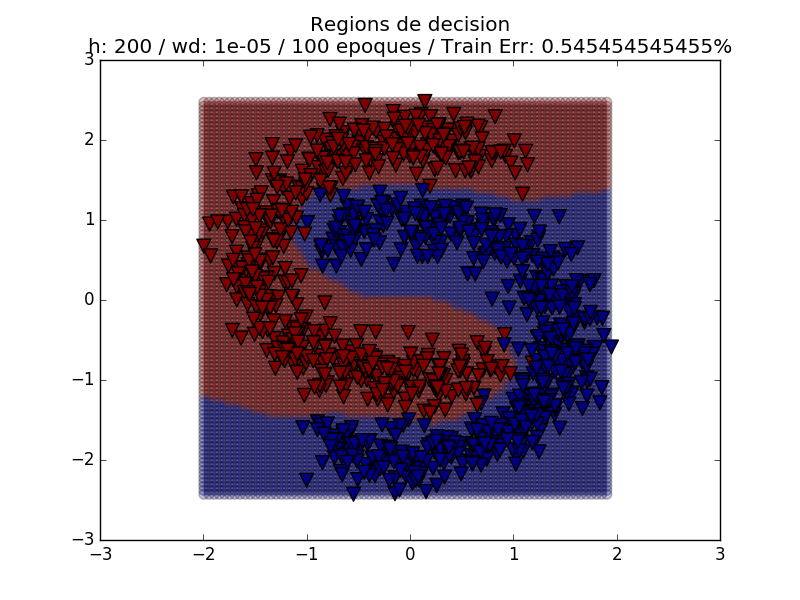
\includegraphics[width=10cm]{images/exo5-under1.png}
	\centering
	\label{fig:comp}
\end{figure}

\todo{1 ou 2 autres exemples et explication}



\subsection{Exercices 6 et 7	}
\subsection{Input}

La fonction $fprop$ et $bprop$ vont recevoir de nouveaux inputs.
Il recevait avant les exemple un par un et ils avaient la forme suivante :
\[
\begin{bmatrix}
    x_{1}  \\
    x_{2}  \\
    \vdots  \\
    x_{d} 
\end{bmatrix}
\]

A la place ils ont maintenant la forme suivante pour un batch de taille K. 

\[
\begin{bmatrix}
    x_{11} & x_{12} & x_{13} & \dots  & x_{1K} \\
    x_{21} & x_{22} & x_{23} & \dots  & x_{2K} \\
    \vdots & \vdots & \vdots & \ddots & \vdots \\
    x_{d1} & x_{d2} & x_{d3} & \dots  & x_{dK}
\end{bmatrix}
\]

Cela de même pour y.

\subsubsection{fprop}


On cherche a obtenir une matrice pour la sortie du même format que l'input. C'est a dire une matrice ou la colonne i correspond aux sorties pour la colonne i de la matrice X.

Il a été nécessaire de modifier la fonction relu et softmax pour qu'elles acceptent des matrices.

Ensuite, il n'a pas fallu modifier w1, w2, b1 ou bien b2.

En effet lorsqu'on multiplie la transposé de X par w1, au lieu d'obtenir un vecteur colonne comme avant, on obtient une matrice de K vecteur colonne. Il suffit de rajouter b1 a chaque colonne ensuite.

Cela de même pour oa, au lieu d'obtenir un vecteur colonne, on obtient la matrice des K vecteurs colonnes.


Il suffit ensuite d'appliquer le softmax modifier pour accepter la matrice.
\subsubsection{bprop}

\todo{ici}

\subsubsection{Verification des modifications}
Pour cette question, on a écrit une méthode qui pour deux réseaux de neurones vérifie que les gradients soient équivalent. C'est a dire qui va regardé pour deux classe NeuralNetwork que les quatre attributs de classes (gradw1, gradw2, gradb1, gradb2) sont égales. Il faut bien sur initialiser les matrices w1 et w2 à des mêmes valeurs.

Pour vérifier que les gradients soient équivalents, on commence par instancier les deux classes correspondant aux deux implémentations $NeuralNetwork$ et $NeuralNetworkEfficient$. On initie ensuite $W1$ et $W2$ des deux classes aux mêmes valeurs. Ensuite on execute l'entrainement pour K=1. On utilise ensuite la méthode qui pour deux réseaux de neurones vérifie que les gradients soient équivalent. On recommence le procédé pour K=10.

Les tests de comparaison nous donne (ok signifie que les deux gradients sont égaux):

\begin{verbatim}
--- K=1 ---
Test Ok : gradient b2
Test Ok : gradient w2
Test Ok : gradient b1
Test Ok : gradient w1
 --- K=10 ---
Test Ok : gradient b2
Test Ok : gradient w2
Test Ok : gradient b1
Test Ok : gradient w1
\end{verbatim}


\subsection{Exercices 8}

Les résultats des mesures de temps sont les suivant : 

\begin{verbatim}
>>EXERCICE 8 MNIST
--- Reseau de depart ---
Cela a mis : 0.419163 secondes
--- Reseau optimise ---
Cela a mis : 0.123445 secondes
\end{verbatim}

Sur cette exécution, on remarque que le temps d'exécution sur le réseau avec matrice est entre 3 et 4 fois plus rapide que sur le réseau avec boucles. Le gain de performance n'est donc pas négligeable.
Si on essaye d'autres exécutions, on remarque des résultats similaires.

\subsection{Exercices 9 et 10}

\end{document}
